\documentclass[a4paper]{ctexart}
\usepackage{xeCJK}
\usepackage{setspace}
\usepackage{graphicx,wrapfig}
\usepackage{fontspec,xunicode,xltxtra}
\usepackage{fancyhdr,titlesec,titletoc}
\usepackage[titletoc]{appendix}
\usepackage[top=29mm,bottom=29mm,left=31.8mm,right=31.8mm]{geometry}
\usepackage{enumerate,enumitem}
\usepackage{caption,subcaption}
\usepackage{amsmath,amssymb,bm,array}
\usepackage{cite}
\usepackage{diagbox}
\usepackage{algorithm,algorithmicx,algpseudocode}
\usepackage{multirow}
\usepackage[super]{gbt7714}
\setmainfont{Times New Roman}
\setCJKmainfont[BoldFont={Songti SC Bold}]{SimSun}
\setCJKfamilyfont{heiti}{SimHei}
\renewcommand{\heiti}{\CJKfamily{heiti}\fontspec{Times New Roman}}
\renewcommand{\appendixpagename}{附录}

\usepackage{listings}
\usepackage[usenames,dvipsnames]{color}
\definecolor{MyDarkGreen}{rgb}{0.0,0.4,0.0}
\lstloadlanguages{Matlab}
\lstset{language=Matlab,
        frame=single,
        basicstyle=\small\ttfamily,
        keywordstyle=[1]\color{Blue}\bfseries,
        keywordstyle=[2]\color{Purple},
        keywordstyle=[3]\color{Blue}\underbar,
        identifierstyle=,
        commentstyle=\usefont{T1}{pcr}{m}{sl}\color{MyDarkGreen}\small,
        stringstyle=\color{Purple},
        showstringspaces=false,
        tabsize=5,
        morekeywords={xlim,ylim,var,alpha,factorial,poissrnd,normpdf,normcdf},
        morekeywords=[2]{on, off, interp},
        morekeywords=[3]{FindESS, homework_example},
        morecomment=[l][\color{Blue}]{...},
        numbers=left,
        firstnumber=1,
        numberstyle=\tiny\color{Blue},
        stepnumber=5
        }
\newcommand{\matlabscript}[2]
  {\begin{itemize}\item[]\lstinputlisting[caption=#2,label=#1]{#1.m}\end{itemize}}

\newcommand{\mycaptionfont}{\heiti\zihao{5}}
\captionsetup[figure]{name={\mycaptionfont 图},labelsep=period}
\captionsetup[table]{name={\mycaptionfont 表},labelsep=period}
\floatname{algorithm}{\mycaptionfont 算法}
\captionsetup[algorithm]{labelsep=period}
\renewcommand{\captionfont}{\mycaptionfont}
\renewcommand{\captionlabelfont}{\mycaptionfont}

\ctexset {
	section = {
		number = \arabic{section},
		format = \zihao{4}\bfseries,
	},
	subsection = {
		number = \arabic{section}.\arabic{subsection},
		format = \zihao{-4}\bfseries,
	},
	subsubsection = {
		number = \arabic{section}.\arabic{subsection}.\arabic{subsubsection},
		format = \zihao{-4}\bfseries,
	}
}
\setlist[enumerate]{itemindent=2em,listparindent=2em,leftmargin=0em,label=\arabic*、}

\setlength\parskip{.5\baselineskip}
\fancypagestyle{plain}{\pagestyle{fancy}}%改变章节首页页眉
\pagestyle{fancy}
\lhead{\kaishu~RFID无线射频识别实验报告~}
\rhead{\kaishu~1030616134~尹达恒}
\cfoot{\thepage}

\begin{document}

\begin{center}
	{\zihao{-3}\textbf{实验三\quad MATLAB编程实现二进制树搜索}}

	{\zihao{-4}尹达恒}\\[-1mm]

	{\zihao{5}(江南大学物联网工程学院,江苏\quad 无锡)}
\end{center}

\renewcommand{\baselinestretch}{1.3}
\zihao{-4}
\section{实验目的}
通过本次实验,了解二进制树搜索理论,再进一步了解其的改进型二进制搜索理论,并将理论知识与实际相结合。

\section{实验设备}
MATLAB编程软件

\section{实验原理}\label{实验原理}
二进制搜索技术以唯一的序列号来识别射频电子标签为基础。为了从一簇射频电子标签中选择其中之一, 射频读写器发出一个读命令, 将射频电子标签序列号传输时的数据碰撞引导到射频读写器, 即由射频读写器判断是否有碰撞发生。 如果有, 则进一步搜索。在二进制算法的实现中, 起决定作用的是射频读写器所使用的信号编码必须能够确定碰撞发生的准确位置。

“二进制树搜索”算法是由在一个射频读写器和多个射频电子标签之间规定的相互作用(命令和应答)顺序(规则)构成的,目的在于从较大的一组中选出一个标签。算法规定,射频电子标签之间要严格同步,以便准确地监测碰撞位的发生,并且要求能辨认出读写器中数据碰撞的比特位的准确位置,一般采用曼切斯特编码。

为了实现这种算法,就需要一组命令,这组命令由射频读写器发出,可由射频电子标签处理,命令如下:
\begin{itemize}
	\item {\bfseries REQUEST}:此命令发送一序列号作为参数给射频电子标签。射频电子标签把自己的序列号与接收的序列号比较。如果小于或等于请求序列号,则此射频电子标签回送其序列号给射频读写器。这样就可以缩小预选的射频电子标签的范围请求;
	\item {\bfseries SELECT}:用某个事先确定的序列号作为参数发送给射频电子标签。具有相同序列号的射频电子标签将此作为执行其他命令(例如读出和写入数据)的切入开关, 选择这个射频电子标签。具有其他序列号的射频电子标签只对REQUEST命令应答;
	\item {\bfseries READ-DATA}:选中的射频电子标签将其存储的数据发送给射频读写器;
	\item {\bfseries UNSELECT}:取消一个选中的射频电子标签,使射频电子标签进入“静默”状态, 这种状态中电于标签完全是非撤活的,对收到的REQUEST命令不作应答。为了更新激活射频电子标签,暂时离开射频读写器的作用范围(等于没有供应电压),以实现复位。
\end{itemize}\subsection{普通的二进制搜索方法}\label{普通的二进制搜索方法}
每个射频电子标签拥有唯一的序列号UID,读写器与多个射频电子标签之间按规定的相互握手(命令和应答)的顺序进行通信,以实现在较大的射频电子标签组中选出所需的射频电子标签。该算法要求读写器能准确辨别碰撞的位置(位检测)。

\subsection{二分支搜索方法}\label{二分支搜索方法}
该方法采用递归的工作方式,遇到碰撞就随机地进行分支,成为多个子集。在接下来的时隙中,主要解决信息包所发生的碰撞。如果再次发生碰撞,就继续随机地分为多个分支。然后依次进行查询,标签被分支后,由于响应的标签数量减少,再次发生碰撞的概率降低,通过不断的分支,减少响应标签的数量,直至分支内没有或仅有一个标签响应。

\section{实验步骤}
\subsection{普通二进制搜索方法}
按照\ref{普通的二进制搜索方法}中的思路,普通二进制搜索方法算法大致过程如下:
\begin{enumerate}
	\item 得到8位二进制数的随机序列,分成25份;
	\item 先对每一次都找出碰撞的最高位;
	\item 选择比碰撞位小的二进制数,然后继续进行第②步骤,直至选择出最小的那一个;
	\item 去除最小的那一行,在进行第二三四步的循环,并记下用时;
	\item 画出曲线图。
\end{enumerate}
按照上述思路编写代码(见附录),运行结果为:
\begin{lstlisting}
	这8个标签分别为:
	0     1     1     0     1     0     0     1
	0     0     1     1     0     0     0     1
	0     1     0     1     0     0     0     0
	1     0     0     0     0     0     1     1
	0     1     0     1     0     1     0     0
	1     0     0     0     0     0     1     0
	1     1     0     1     0     1     0     1
	1     1     1     0     1     0     0     1

读写器接收到的ID为:     9     9     9     9     9     9     9     9

下一次读写器命令为01111111
读写器接收到的ID为:     0     9     9     9     9     9     0     9

下一次读写器命令为00111111
读写器接收到的ID为:     0     0     1     1     0     0     0     1

标签2已识别
下一次读写器命令为11111111
读写器接收到的ID为:     9     9     9     9     9     9     9     9

下一次读写器命令为01111111
读写器接收到的ID为:     0     1     9     9     9     9     0     9

下一次读写器命令为01011111
读写器接收到的ID为:     0     1     0     1     0     9     0     0

下一次读写器命令为01010011
读写器接收到的ID为:     0     1     0     1     0     0     0     0

标签3已识别
下一次读写器命令为11111111
读写器接收到的ID为:     9     9     9     9     9     9     9     9

下一次读写器命令为01111111
读写器接收到的ID为:     0     1     9     9     9     9     0     9

下一次读写器命令为01011111
读写器接收到的ID为:     0     1     0     1     0     1     0     0

标签5已识别
下一次读写器命令为11111111
读写器接收到的ID为:     9     9     9     9     9     9     9     9

下一次读写器命令为01111111
读写器接收到的ID为:     0     1     1     0     1     0     0     1

标签1已识别
下一次读写器命令为11111111
读写器接收到的ID为:     1     9     9     9     9     9     9     9

下一次读写器命令为10111111
读写器接收到的ID为:     1     0     0     0     0     0     1     9

下一次读写器命令为10000010
读写器接收到的ID为:     1     0     0     0     0     0     1     0

标签6已识别
下一次读写器命令为11111111
读写器接收到的ID为:     1     9     9     9     9     9     9     1

下一次读写器命令为10111111
读写器接收到的ID为:     1     0     0     0     0     0     1     1

标签4已识别
下一次读写器命令为11111111
读写器接收到的ID为:     1     1     9     9     9     9     0     1

下一次读写器命令为11011111
读写器接收到的ID为:     1     1     0     1     0     1     0     1

标签7已识别
下一次读写器命令为11111111
读写器接收到的ID为:     1     1     1     0     1     0     0     1

标签8已识别
\end{lstlisting}

\subsection{二分支搜索方法}
按照\ref{二分支搜索方法}中的思路,二分支搜索方法大致过程如下:
\begin{enumerate}
	\item 先随机生成16位的标签号,定义标签的左右子树;
	\item 先找出标签碰撞的位数,若得到碰撞的位,根据碰撞的位将标签号分为左右两子树(定义左子树位1,右子树位0);
	\item 判断左子树是否只有一个标签或无标签,若是,则该次调用结束,判断上步的右子树是否只有一个标签或无标签,若不是,则进入该右子树的左子树进行查验,以此循环。
\end{enumerate}
按照上述过程编写代码,并将程序嵌入到Matlab图形界面中,运行结果如图\ref{fig:3}
\begin{figure}[htbp]
	\centering
	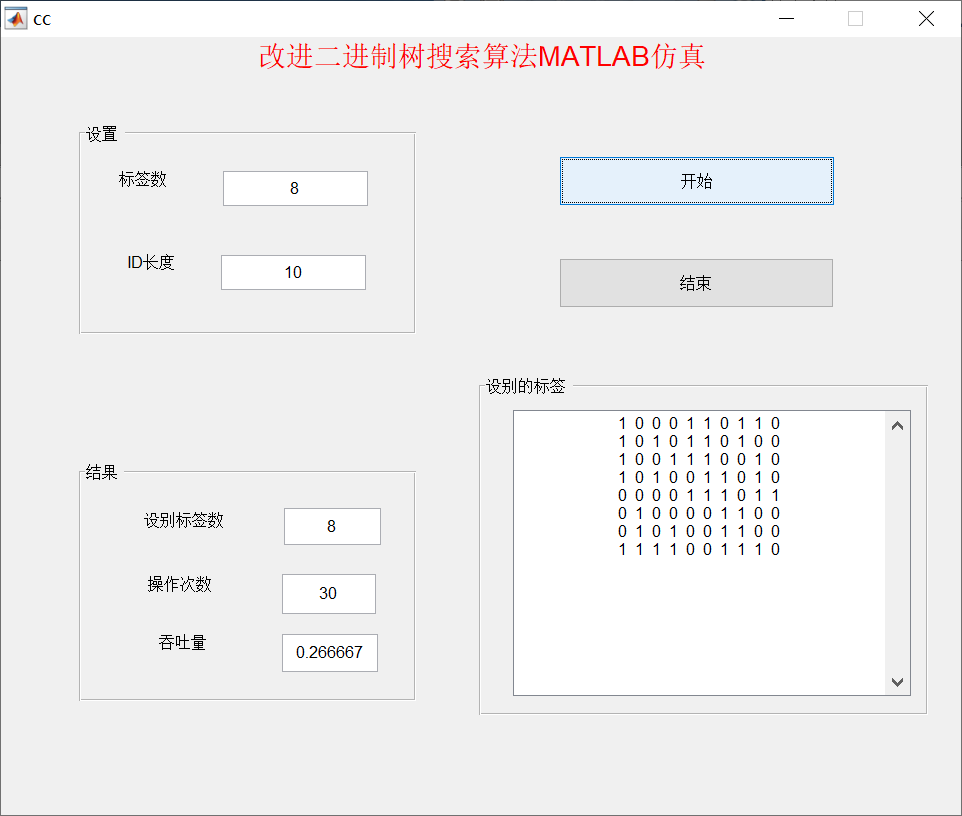
\includegraphics[width=0.8\textwidth]{figure/1.png}
	\caption{二分支搜索方法模拟结果}\label{fig:3}
\end{figure}

\newpage
\appendix
\appendixpage
\section{普通的二进制搜索方法实验代码}
\begin{lstlisting}
N=4;%标签数目
IDs=zeros([N,8]);
OKs=zeros([1,N]);
for i=1:N
IDs(i,:)=(rand([1,8])>0.5);
end
fprintf('这%d个标签分别为:\n',N);
disp(IDs);

total=N;
request=ones([1,8]);
response=zeros([1,8]);
while sum(OKs)<N
    s=1;
    val=zeros([1,N]);
    for i=1:N
        if OKs(i)<1
            for j=1:8
                if IDs(i,j)<=request(j)
                    val(i)=val(i)+1;
                end
            end
            if val(i)==8
                if i~=1&&sum(val(1:i-1)==8)>0
                    response(response~=IDs(i,:))=9;
                else
                    response=IDs(i,:);
                end
            end
        end
    end
    fprintf('读写器接收到的ID为:');
    disp(response);
    fprintf('\n');
    for i=1:N
        if response==IDs(i,:)
            fprintf('标签%d已识别\n',i);
            OKs(i)=1;
            request=ones([1,8]);
            total=total-1;
            break;
        end
    end
    if total~=0
        for j=1:1:8
            if response(j)~=9
                request(j)=response(j);
            elseif response(j)==9
                request(j)=0;
                s=j+1;
                break
            end
        end
        for j=s:1:8
            request(j)=1;
        end
        fprintf('下一次读写器命令为');
        for i=1:1:8
            fprintf('%d',request(i));
        end
        fprintf('\n');
    end
end
\end{lstlisting}
\section{二分支搜索方法核心代码}
\begin{lstlisting}
function c=pick(A,tag_count,b,ID_length)
left_tag(tag_count,ID_length)=0;
m=1;
right_tag(tag_count,ID_length)=0;
n=1;
b=b+2;
D_max=0;
x=0;
if tag_count==1
    c=b;
    return;
end
for j=1:1:ID_length
    sum=0;
    for k=1:tag_count
        sum=sum+A(k,j);
    end
    if sum~=0&&sum~=tag_count
        D_max=j;
        break;
    end
end
for i=1:tag_count
    x=A(i,D_max);
    if x==1
        left_tag(m,:)=A(i,:);
        m=m+1;
    else
        right_tag(n,:)=A(i,:);
        n=n+1;
    end
end
if m==2||m==1
    b=b+2;
    c=b;
else
    b=pick(left_tag,m-1,b,ID_length);
end

if n==2||n==1
    b=b+2;
    c=b;  
else
    b=pick(right_tag,n-1,b,ID_length);
end
c=b;
return;

\end{lstlisting}
\end{document}